
\begin{document}


\chapter*{Appendix}

\label{chapter:appendix}

This appendix contains plots from the experiments conducted on Scenes 2 and 3.
Note that for Scene 2, the potential fields planner was not able to complete
find a path to the goal on sufficiently many cases and thus results could not
be concluded. This is a consequence of using a potential fields planner, it may
not bring the robot to the goal if it gets stuck in a local minima.

\chapter*{Appendix I\\Results for Scene 2}

\begin{figure}[h!]
    \centering
    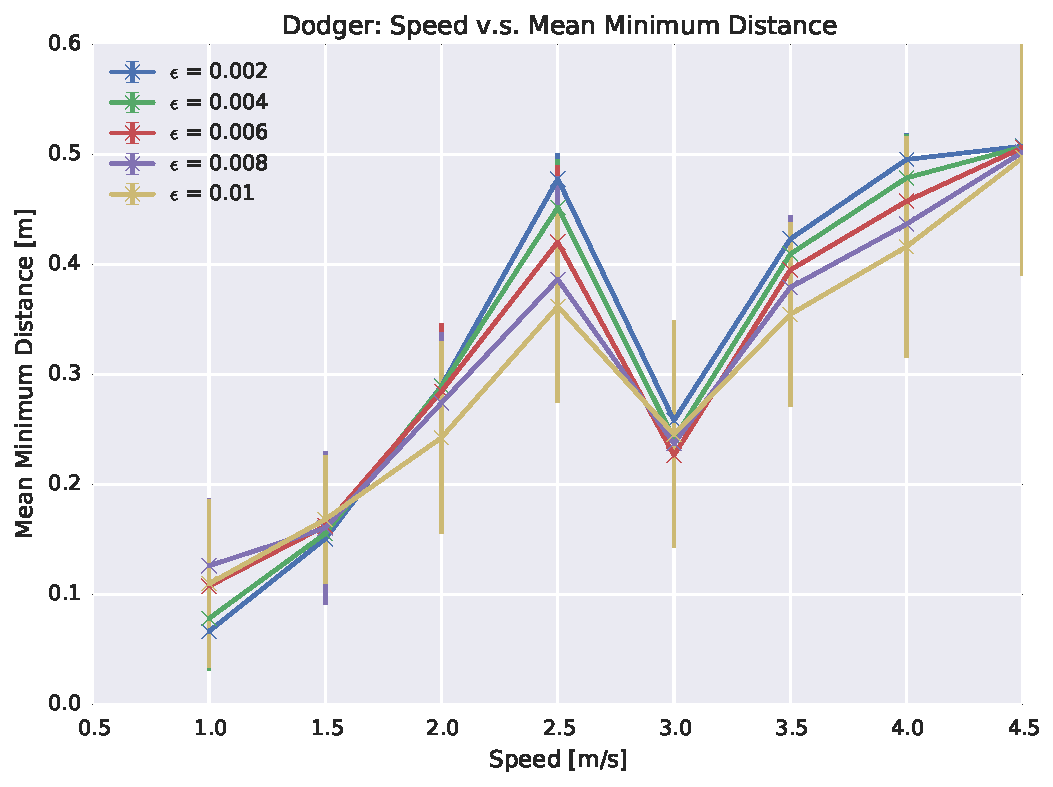
\includegraphics[width=0.80\linewidth]{figs/planner_mean_min_distance_1}

    \caption{Plots showing how the minimum distance to any obstacle for a path
        changes as the speed increases for various amounts of obstacle position
        uncertainties.  The horizontal axis represents the speed of the robot
        and the vertical axis represents the minimum distance to obstacles
        along the path. The different lines on each plot represent experiments
    with differing amounts of noise and the error bars represent one standard
deviation.}

\end{figure}

\begin{figure}[h!]
    \centering

    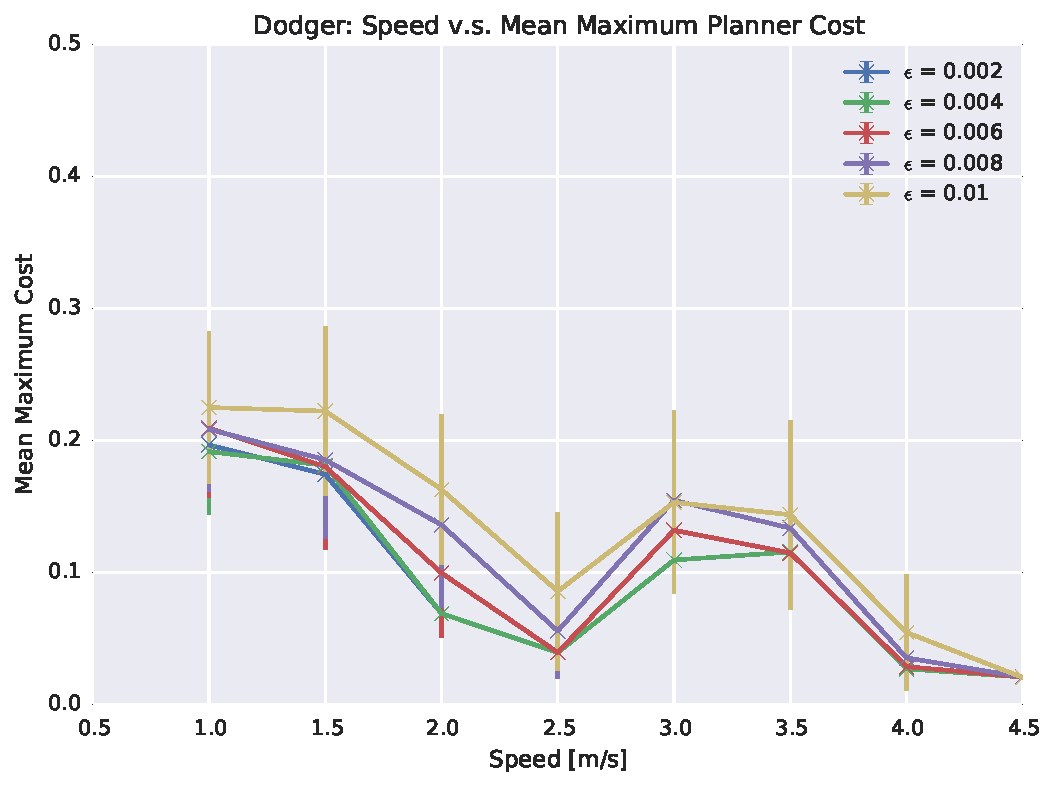
\includegraphics[width=0.80\linewidth]{figs/planner_mean_max_cost_1}

    \caption{Plots showing how the maximum cost for a path changes as the
        speed increases for various amounts of obstacle position uncertainties.
        The horizontal axis represents the speed of the robot and the vertical
        axis represents the maximum cost along the path. The different lines on
    each plot represent experiments with differing amounts of noise and the
error bars represent one standard deviation.}

\end{figure}

\begin{figure}[h!]
    \centering

    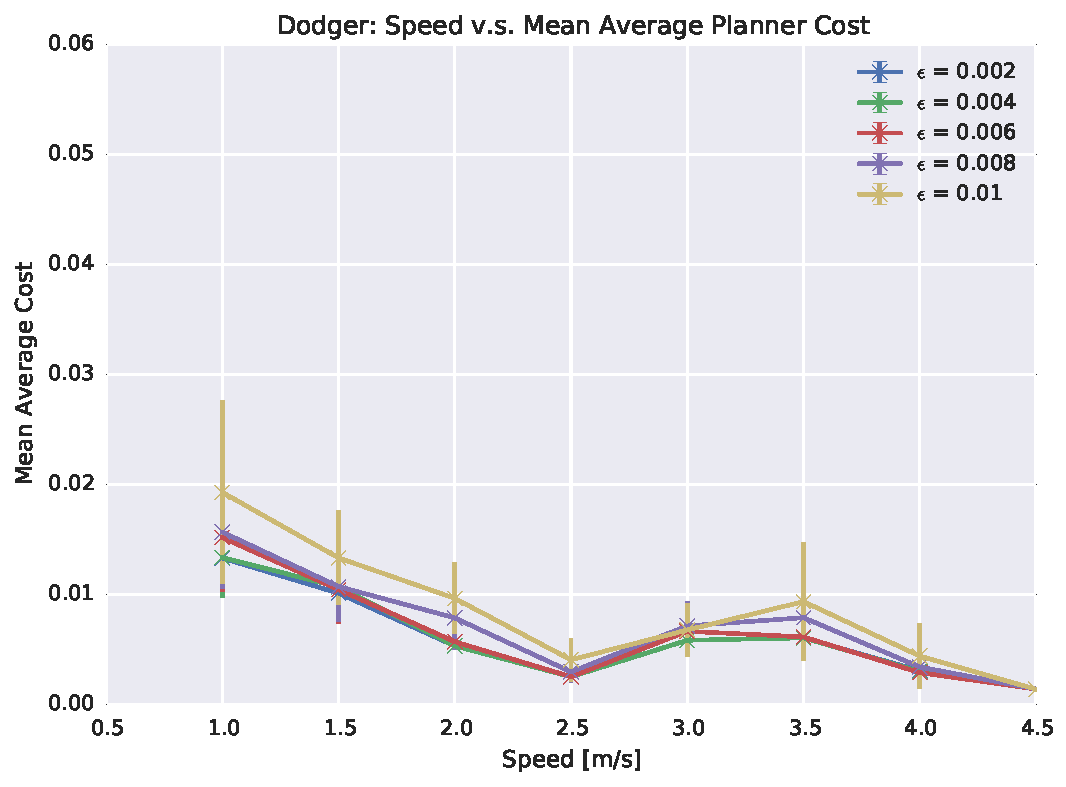
\includegraphics[width=0.80\linewidth]{figs/planner_mean_avg_cost_1}

    \caption{Plots showing how the average cost for a path changes as the
        speed increases for various amounts of obstacle position uncertainties.
        The horizontal axis represents the speed of the robot and the vertical
        axis represents the average cost along the path. The different lines on
    each plot represent experiments with differing amounts of noise and the
error bars represent one standard deviation.}

\end{figure}

\begin{figure}[h!]
    \centering

    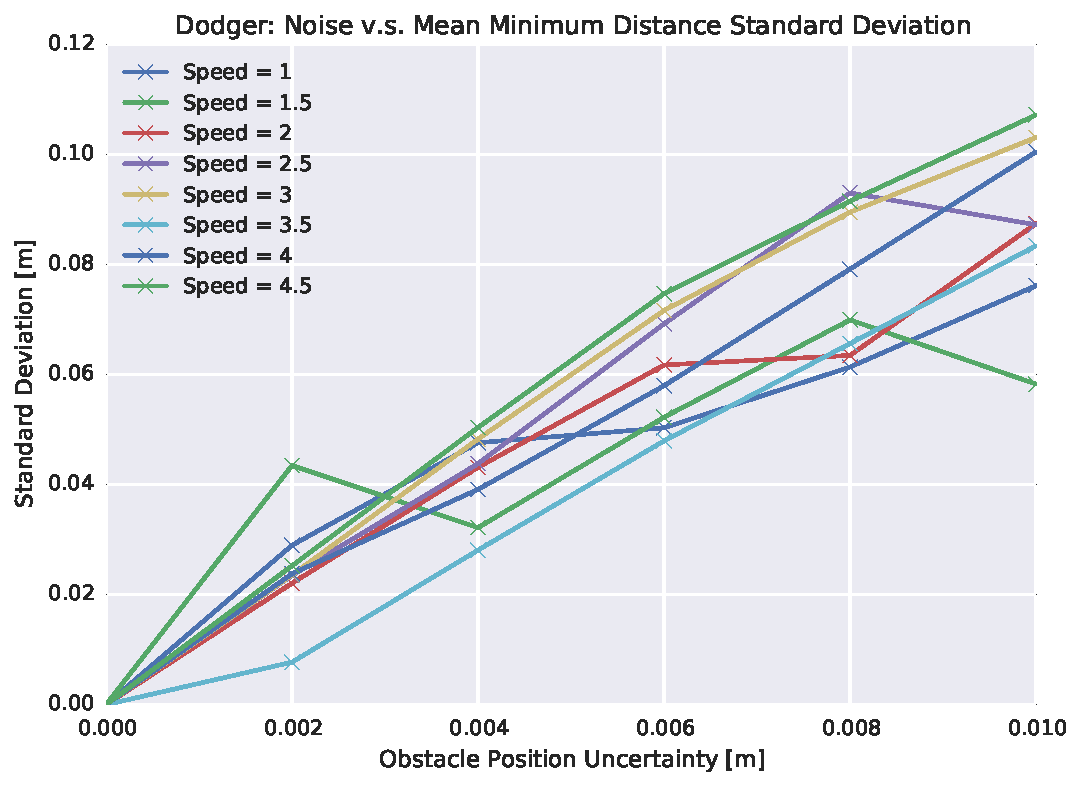
\includegraphics[width=0.80\linewidth]{figs/planner_std_min_distance_1}

    \caption{Plots showing how the standard deviation for the minimum distance
        along a path changes as the noise injected into the obstacle
        trajectories increases. The horizontal axis represents the amount of
        noise and the vertical axis represents the standard deviation. The
        different lines indicate different speeds that the robot was
    travelling.}

\end{figure}

\begin{figure}[h!]
    \centering

    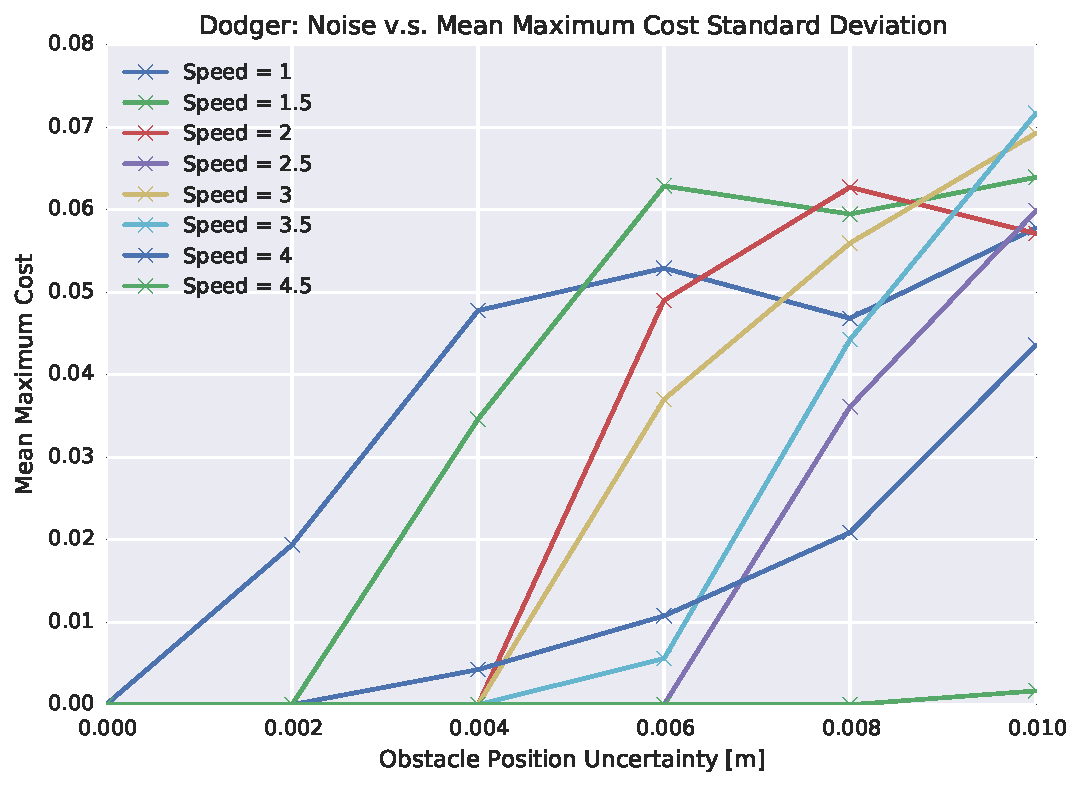
\includegraphics[width=0.48\linewidth]{figs/planner_std_max_cost_1}
    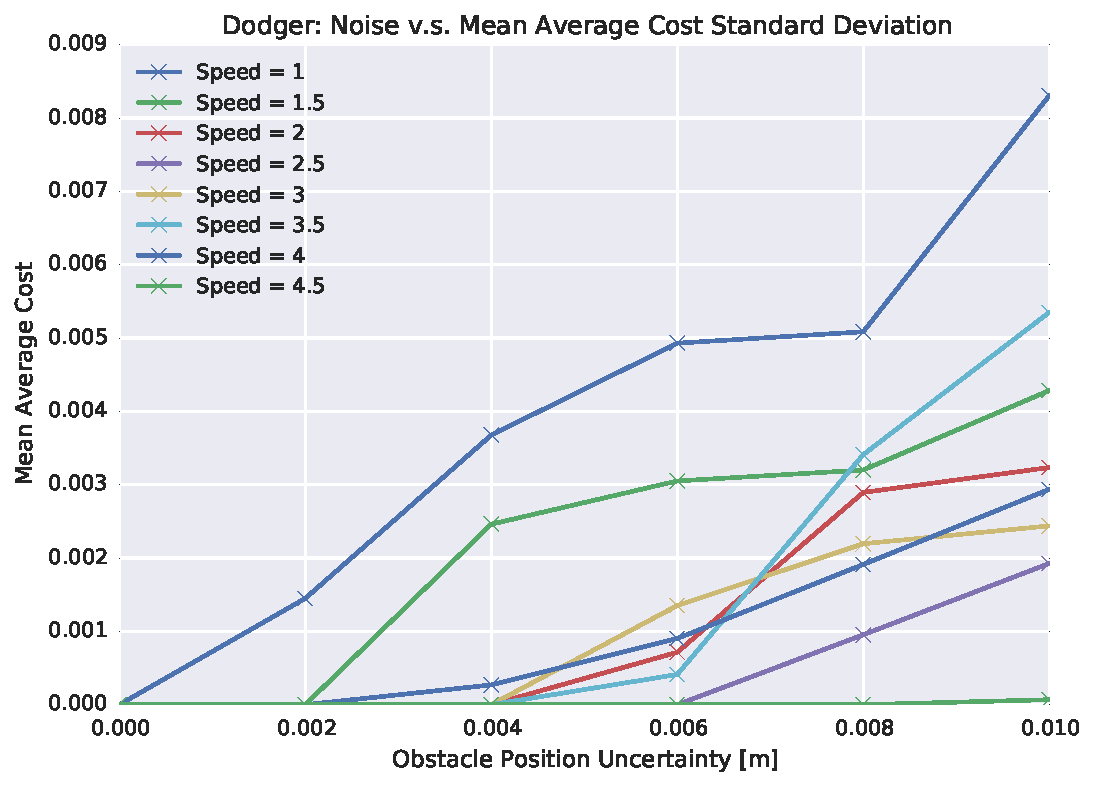
\includegraphics[width=0.48\linewidth]{figs/planner_std_avg_cost_1}

    \caption{Plots showing how the standard deviation for the maximum cost and
        average cost along a path changes as the noise injected into the
        obstacle trajectories increases. The horizontal axis represents the
        amount of noise and the vertical axis represents the standard
        deviation. The different lines indicate different speeds that the robot
        was travelling. On the left is the graph for Dodger and on the right is
    the graph for the potential fields planner.}

\end{figure}

\begin{figure}[h!]
    \centering
    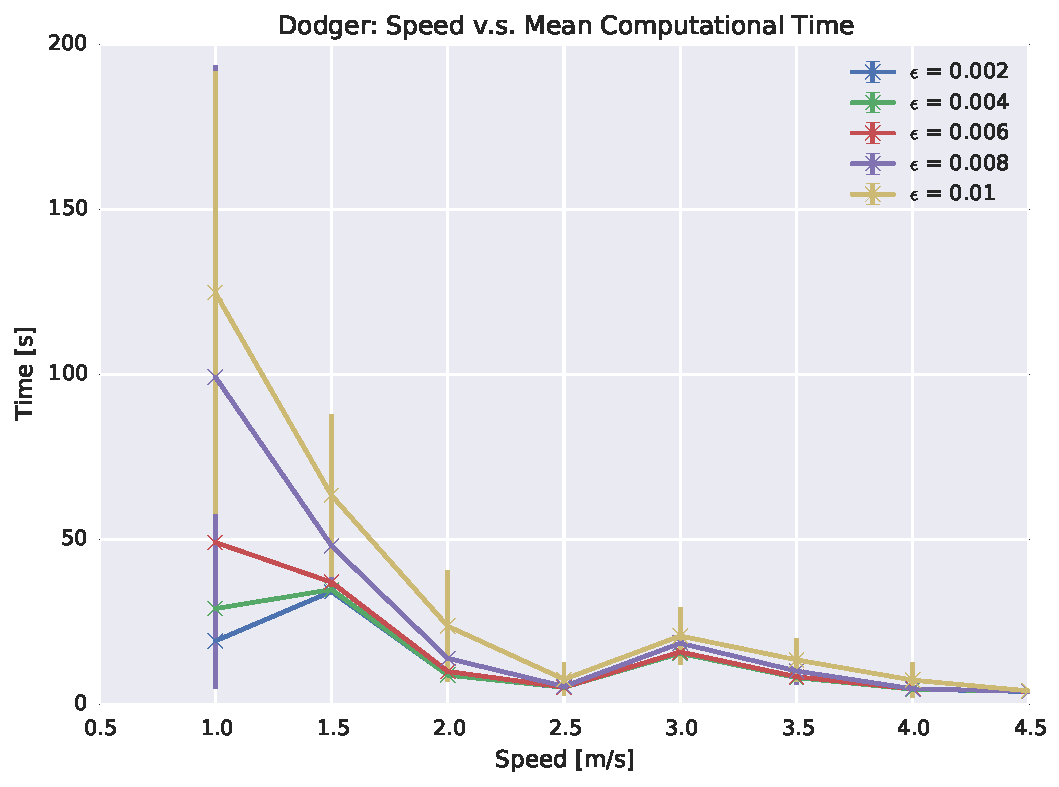
\includegraphics[width=0.48\linewidth]{figs/planner_mean_times_1}
    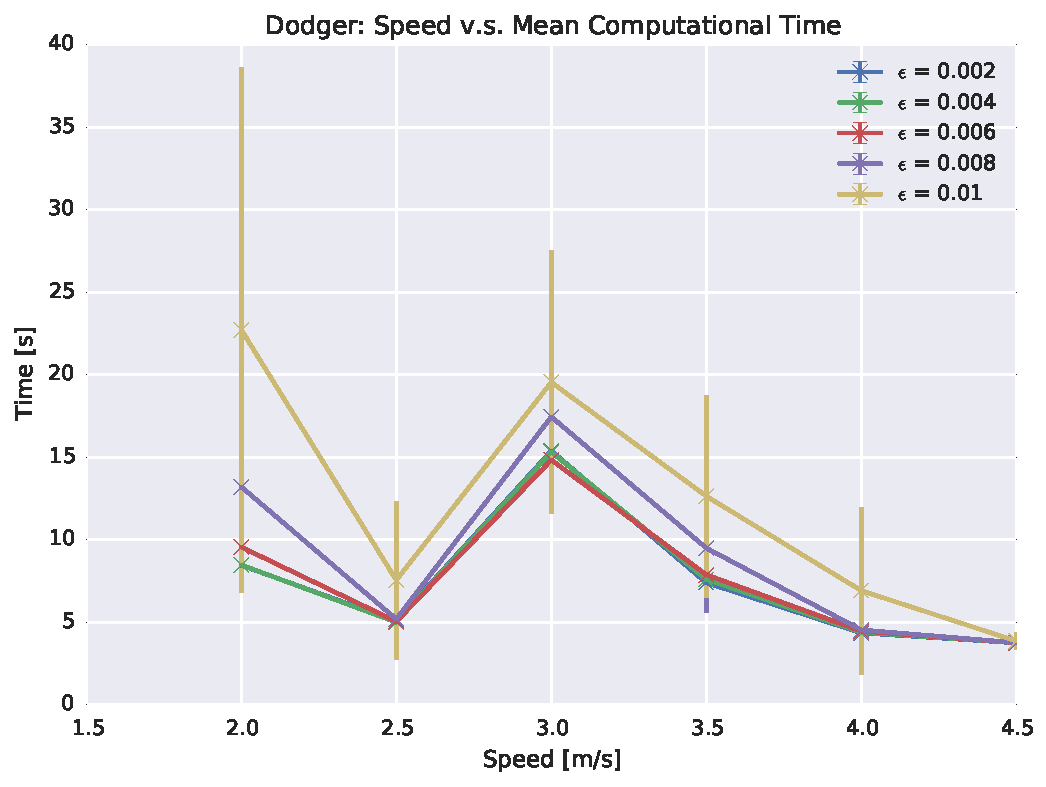
\includegraphics[width=0.48\linewidth]{figs/planner_small_mean_times_1}

    \caption{Plots showing how the computational to generate a path changes as
        the speed increases for various amounts of obstacle position
        uncertainties.  The horizontal axis represents the speed of the robot
        and the vertical axis represents the computational time to generate the
        path. The different lines on each plot represent experiments with
        differing amounts of noise and the error bars represent one standard
        deviation.}

\end{figure}

\begin{figure}[h!]
    \centering

    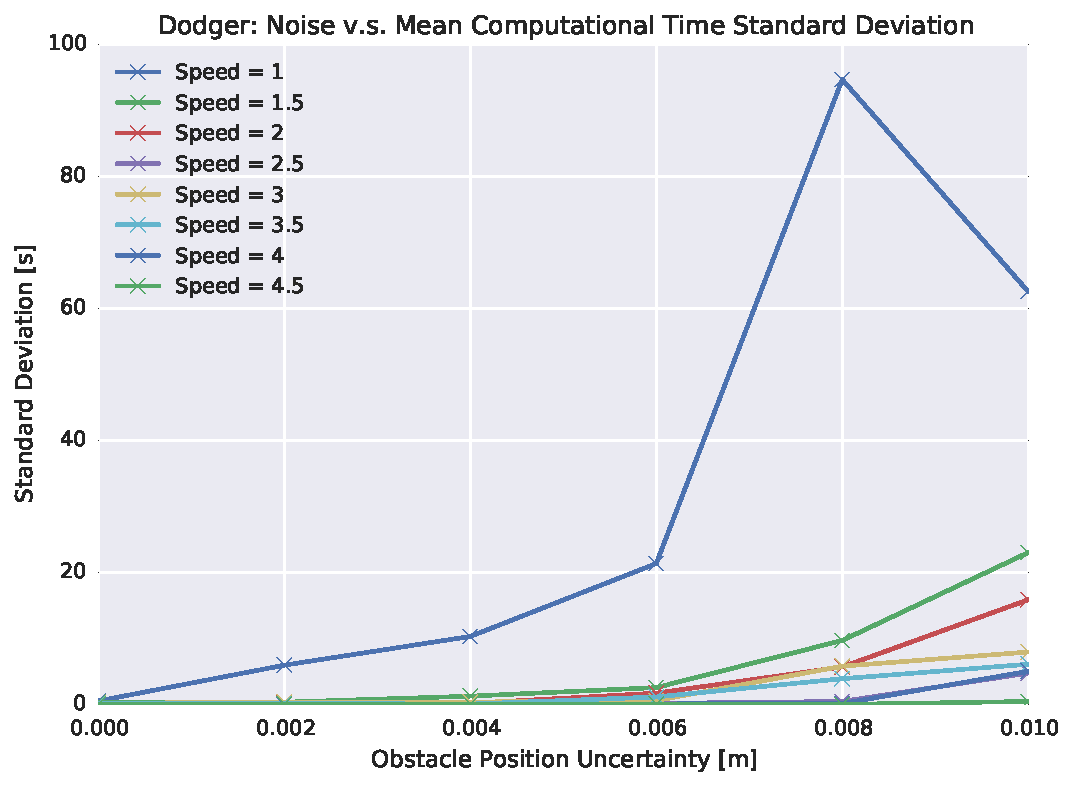
\includegraphics[width=0.80\linewidth]{figs/planner_std_avg_times_1}

    \caption{Plots showing how the standard deviation for the computational
        cost to generate a path changes as the noise injected into the obstacle
        trajectories increases.  The horizontal axis represents the amount of
        noise and the vertical axis represents the standard deviation. The
    different lines indicate different speeds that the robot was travelling.}

\end{figure}

\chapter*{Appendix II\\Results for Scene 3}

\begin{figure}[h!]
    \centering
    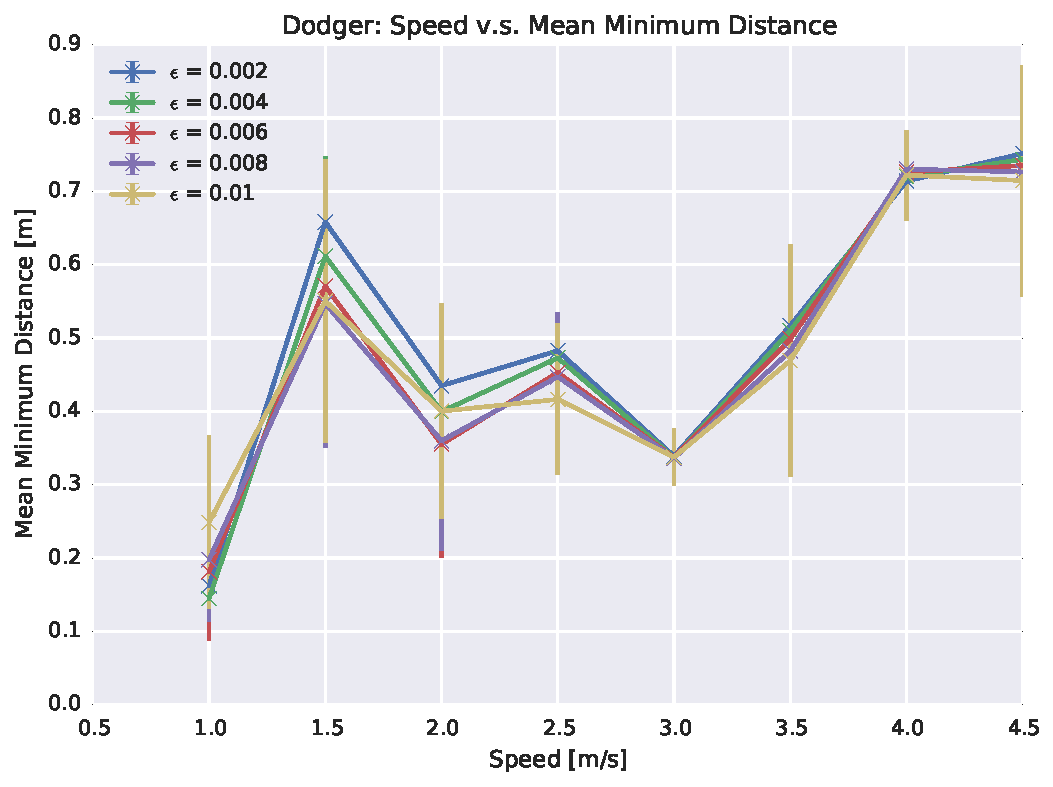
\includegraphics[width=0.48\linewidth]{figs/planner_mean_min_distance_2}
    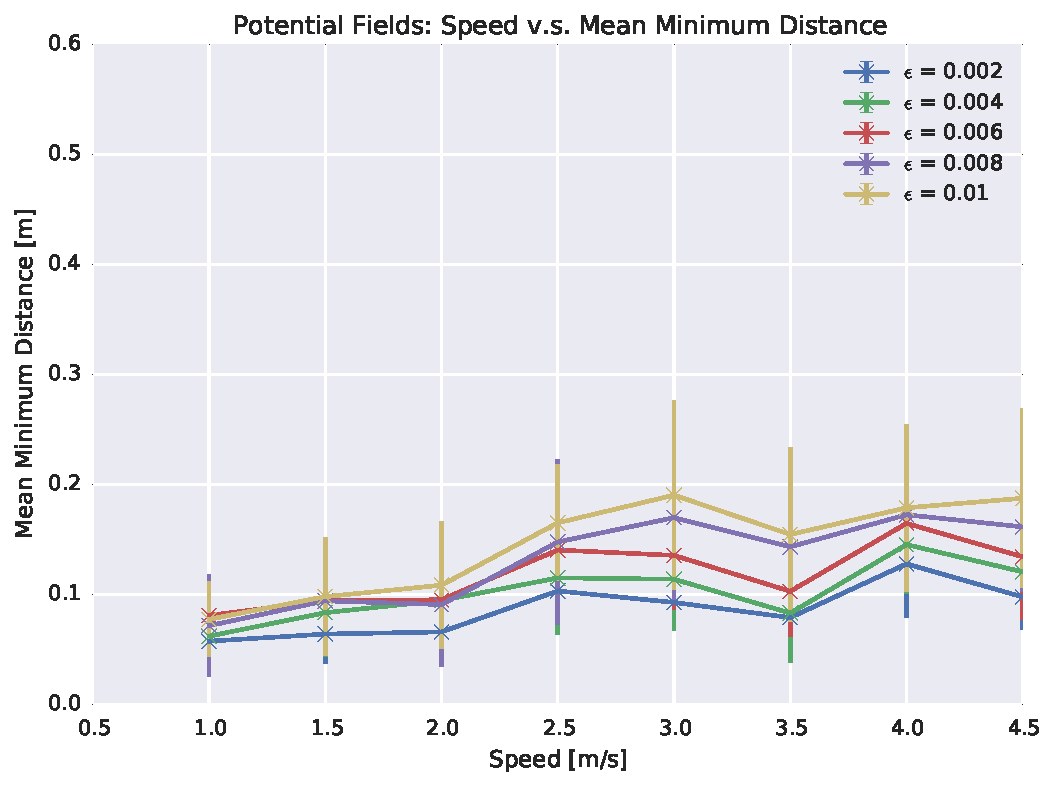
\includegraphics[width=0.48\linewidth]{figs/pf_mean_min_distance_2}

    \caption{Plots showing how the minimum distance to any obstacle for a path
        changes as the speed increases for various amounts of obstacle position
        uncertainties.  The horizontal axis represents the speed of the robot
        and the vertical axis represents the minimum distance to obstacles
        along the path. The different lines on each plot represent experiments
    with differing amounts of noise and the error bars represent one standard
deviation. On the left is the graph for Dodger and on the right is the graph
for the potential fields planner.}

\end{figure}

\begin{figure}[h!]
    \centering

    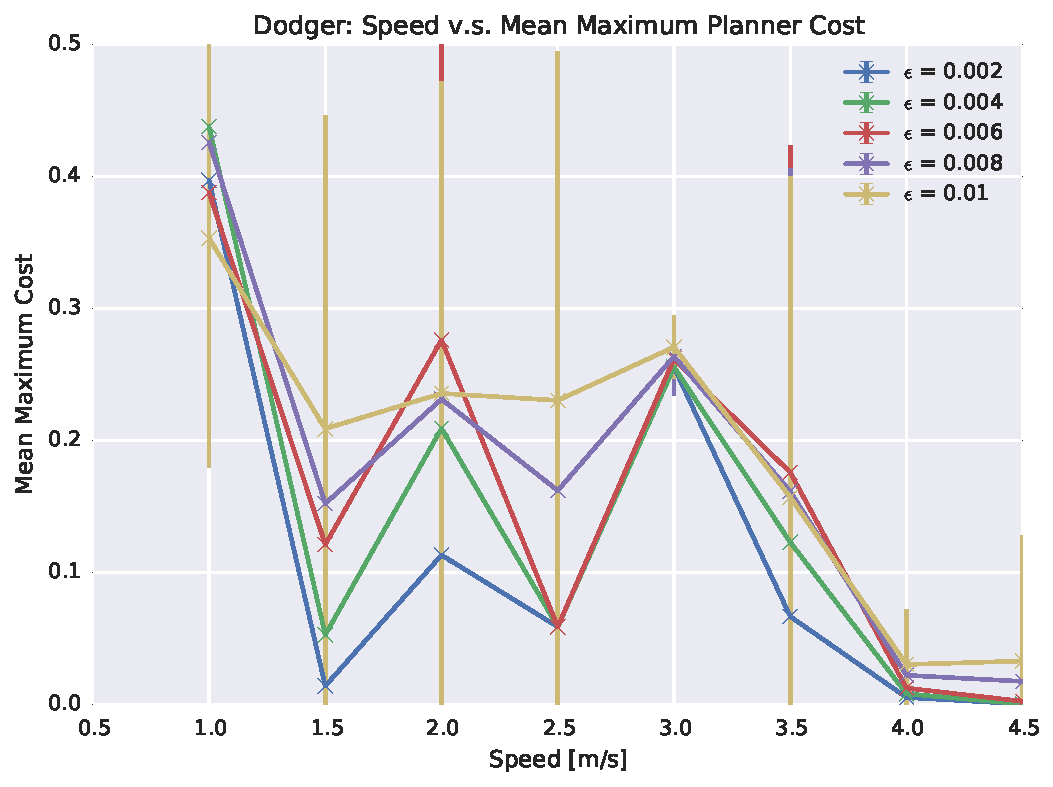
\includegraphics[width=0.48\linewidth]{figs/planner_mean_max_cost_2}
    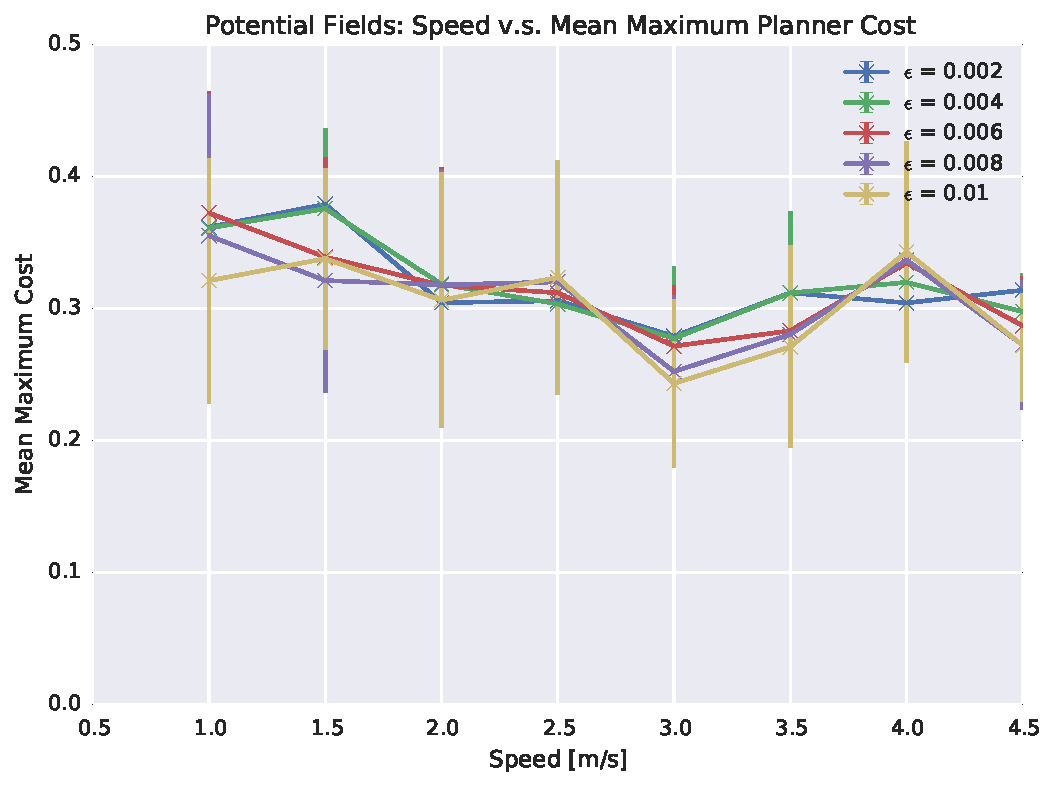
\includegraphics[width=0.48\linewidth]{figs/pf_mean_max_cost_2}

    \caption{Plots showing how the maximum cost for a path changes as the
        speed increases for various amounts of obstacle position uncertainties.
        The horizontal axis represents the speed of the robot and the vertical
        axis represents the maximum cost along the path. The different lines on
    each plot represent experiments with differing amounts of noise and the
error bars represent one standard deviation.  On the left is the graph for
Dodger and on the right is the graph for the potential fields planner.}

\end{figure}

\begin{figure}[h!]
    \centering

    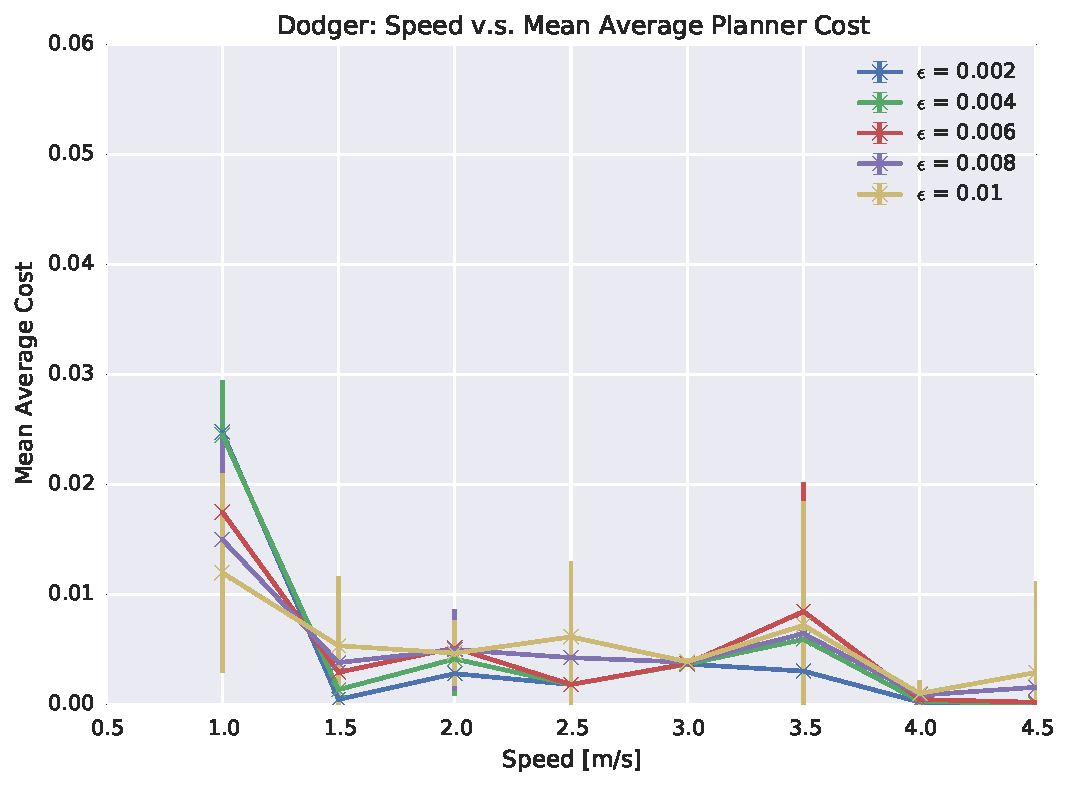
\includegraphics[width=0.48\linewidth]{figs/planner_mean_avg_cost_2}
    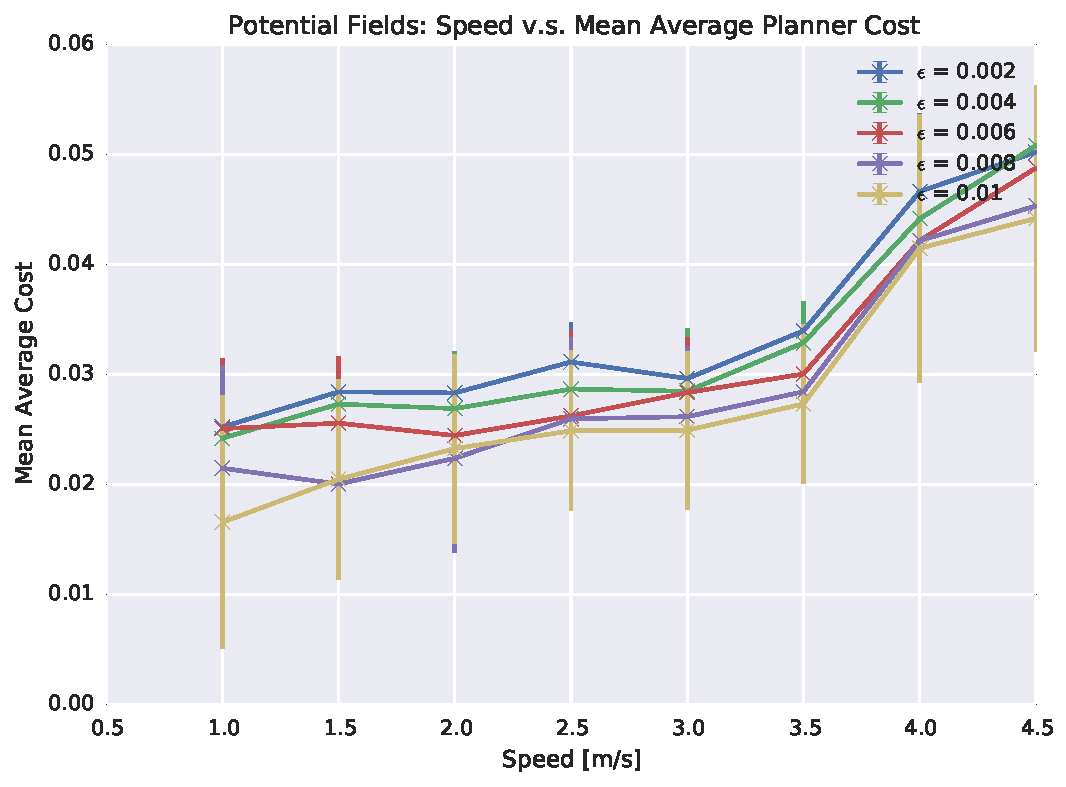
\includegraphics[width=0.48\linewidth]{figs/pf_mean_avg_cost_2}

    \caption{Plots showing how the average cost for a path changes as the
        speed increases for various amounts of obstacle position uncertainties.
        The horizontal axis represents the speed of the robot and the vertical
        axis represents the average cost along the path. The different lines on
    each plot represent experiments with differing amounts of noise and the
error bars represent one standard deviation.  On the left is the graph for
Dodger and on the right is the graph for the potential fields planner.}

\end{figure}

\begin{figure}[h!]
    \centering

    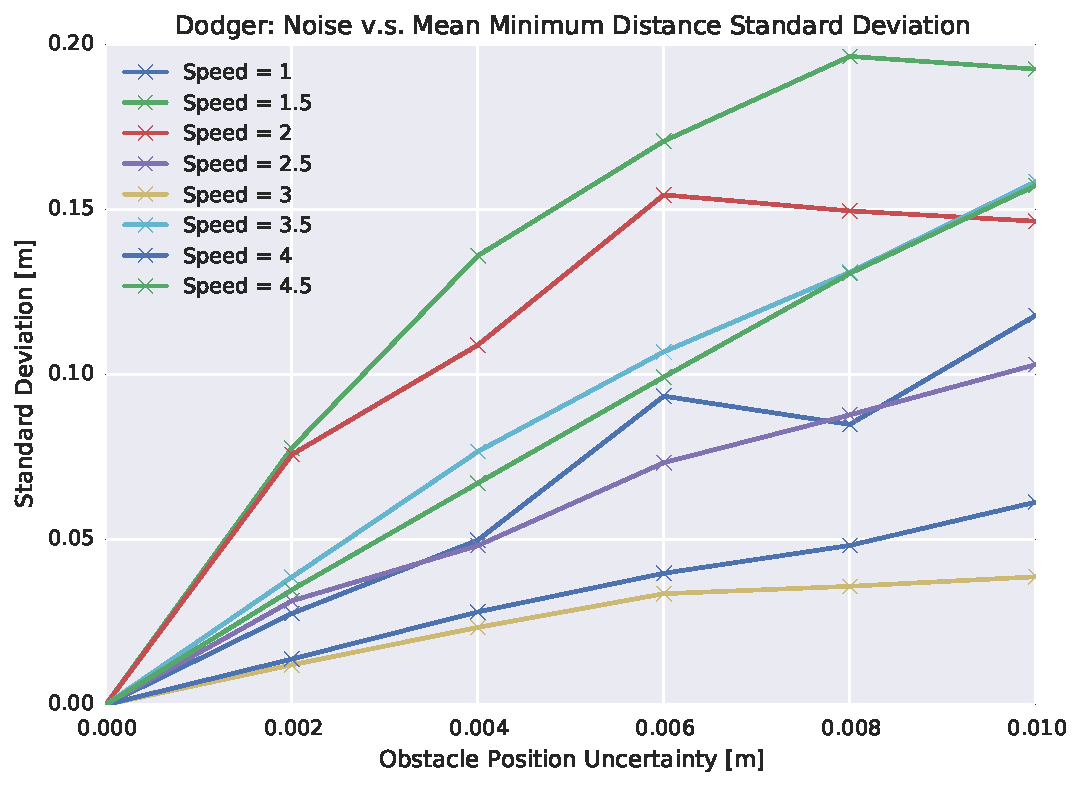
\includegraphics[width=0.48\linewidth]{figs/planner_std_min_distance_2}
    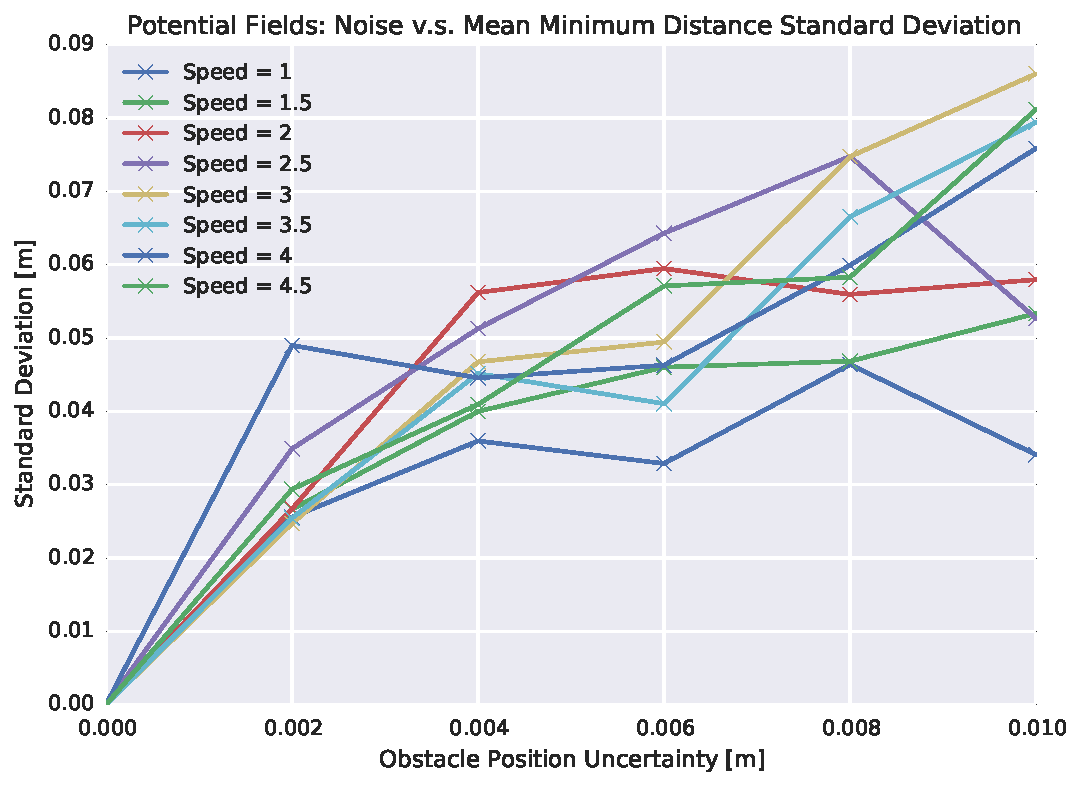
\includegraphics[width=0.48\linewidth]{figs/pf_std_min_distance_2}

    \caption{Plots showing how the standard deviation for the minimum distance
        along a path changes as the noise injected into the obstacle
        trajectories increases. The horizontal axis represents the amount of
        noise and the vertical axis represents the standard deviation. The
        different lines indicate different speeds that the robot was
    travelling. On the left is the graph for Dodger and on the right is the
graph for the potential fields planner.}

\end{figure}

\begin{figure}[h!]
    \centering

    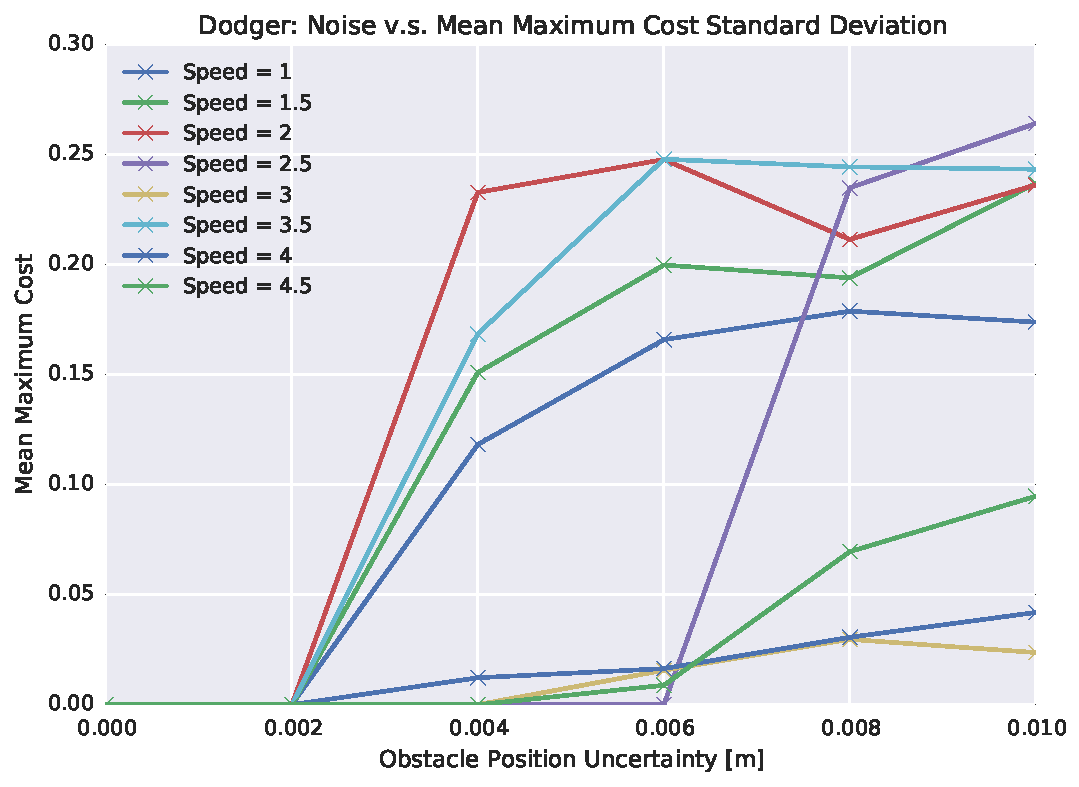
\includegraphics[width=0.48\linewidth]{figs/planner_std_max_cost_2}
    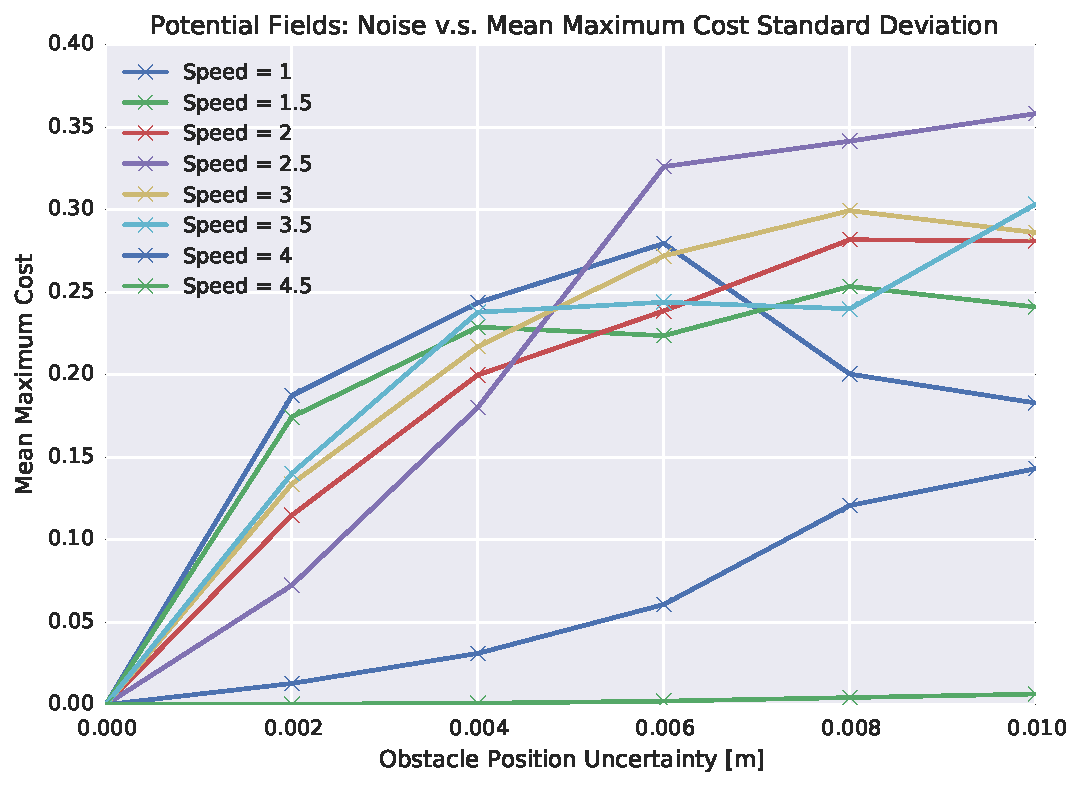
\includegraphics[width=0.48\linewidth]{figs/pf_std_max_cost_2} \\
    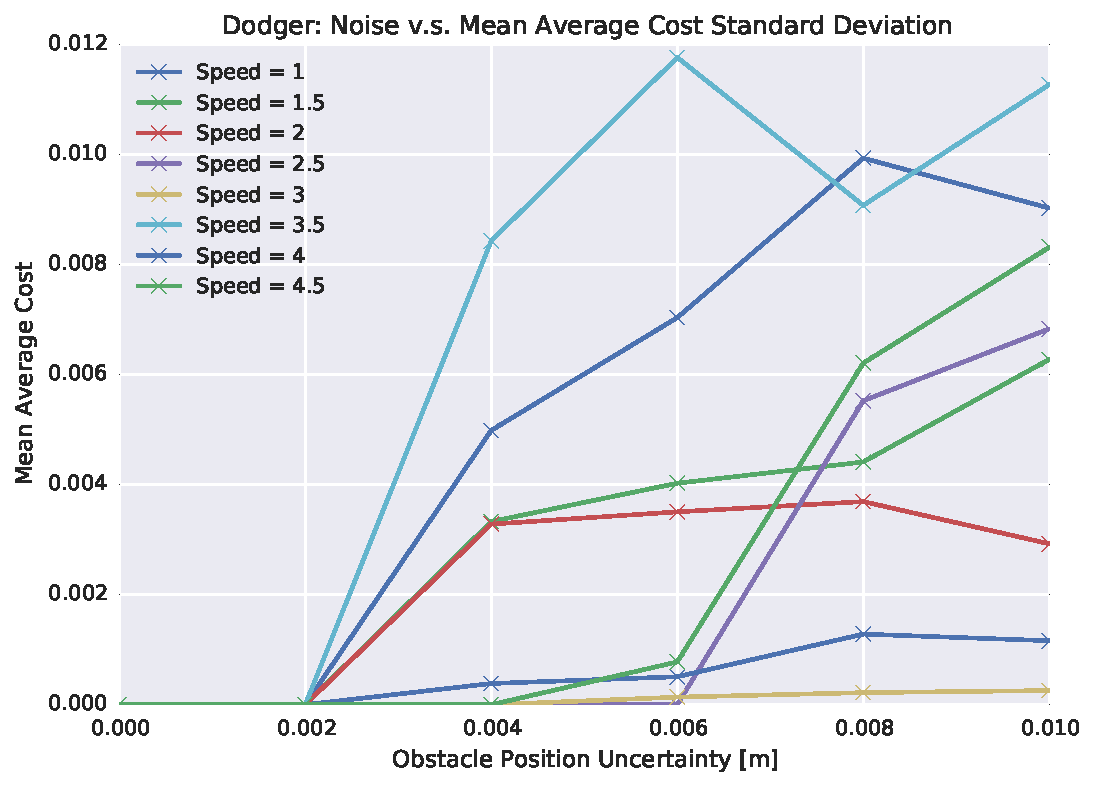
\includegraphics[width=0.48\linewidth]{figs/planner_std_avg_cost_2}
    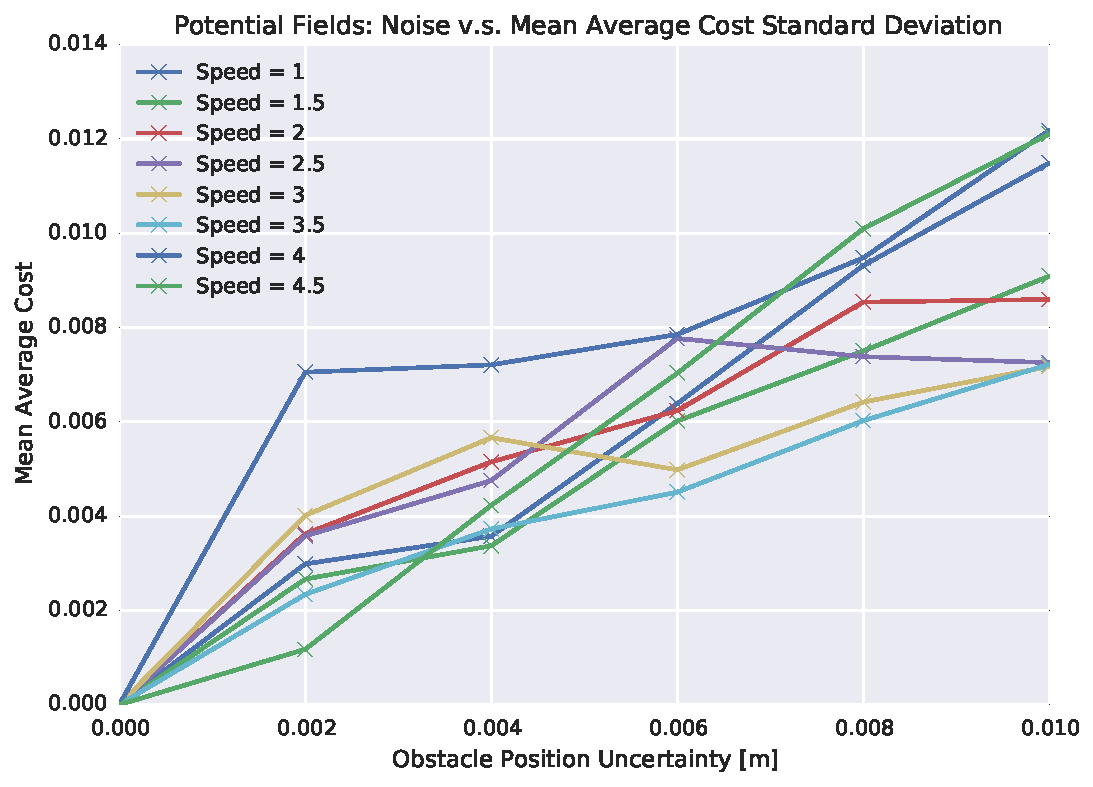
\includegraphics[width=0.48\linewidth]{figs/pf_std_avg_cost_2}

    \caption{Plots showing how the standard deviation for the maximum cost and
        average cost along a path changes as the noise injected into the
        obstacle trajectories increases. The horizontal axis represents the
        amount of noise and the vertical axis represents the standard
        deviation. The different lines indicate different speeds that the robot
        was travelling. On the left is the graph for Dodger and on the right is
    the graph for the potential fields planner. The top row is for the maximum
cost and the bottom row is the for the average cost.}

\end{figure}

\begin{figure}[h!]
    \centering
    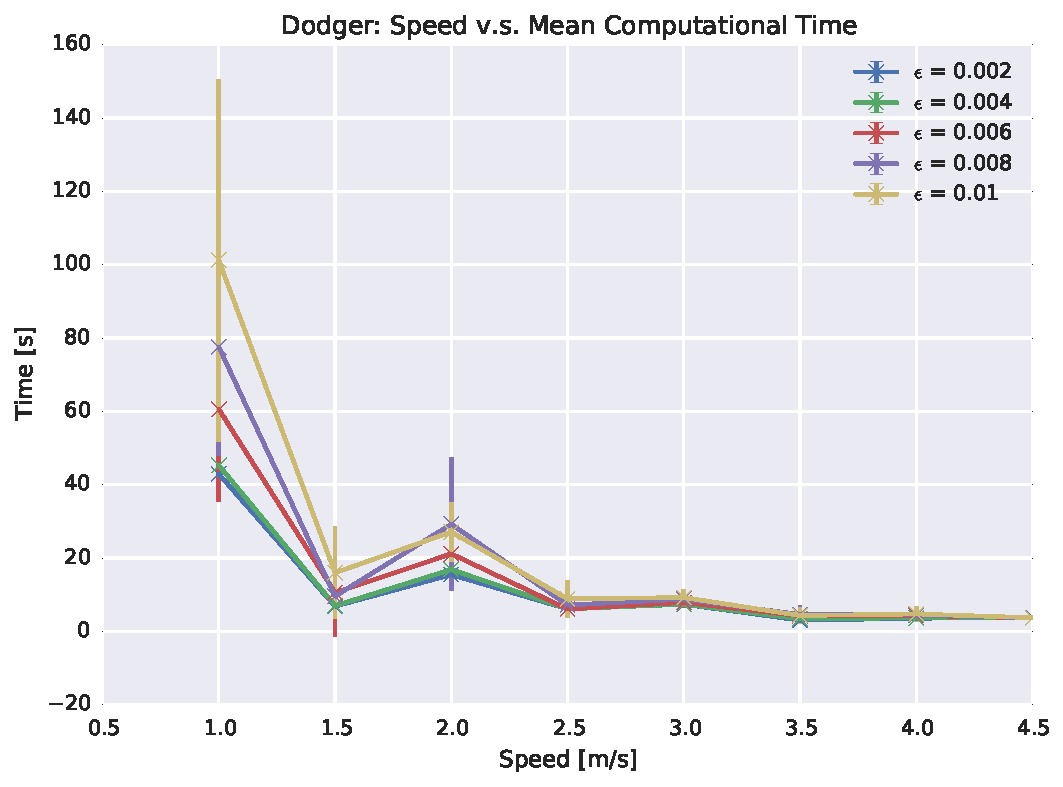
\includegraphics[width=0.48\linewidth]{figs/planner_mean_times_2}
    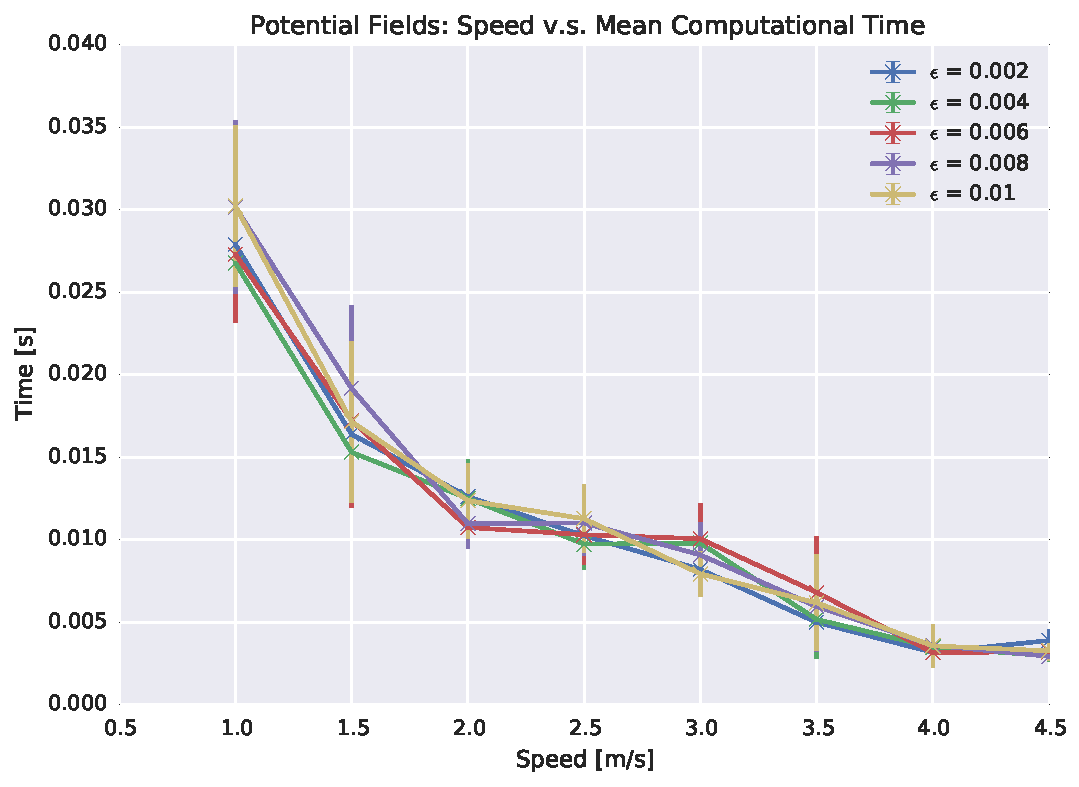
\includegraphics[width=0.48\linewidth]{figs/pf_mean_times_2} \\
    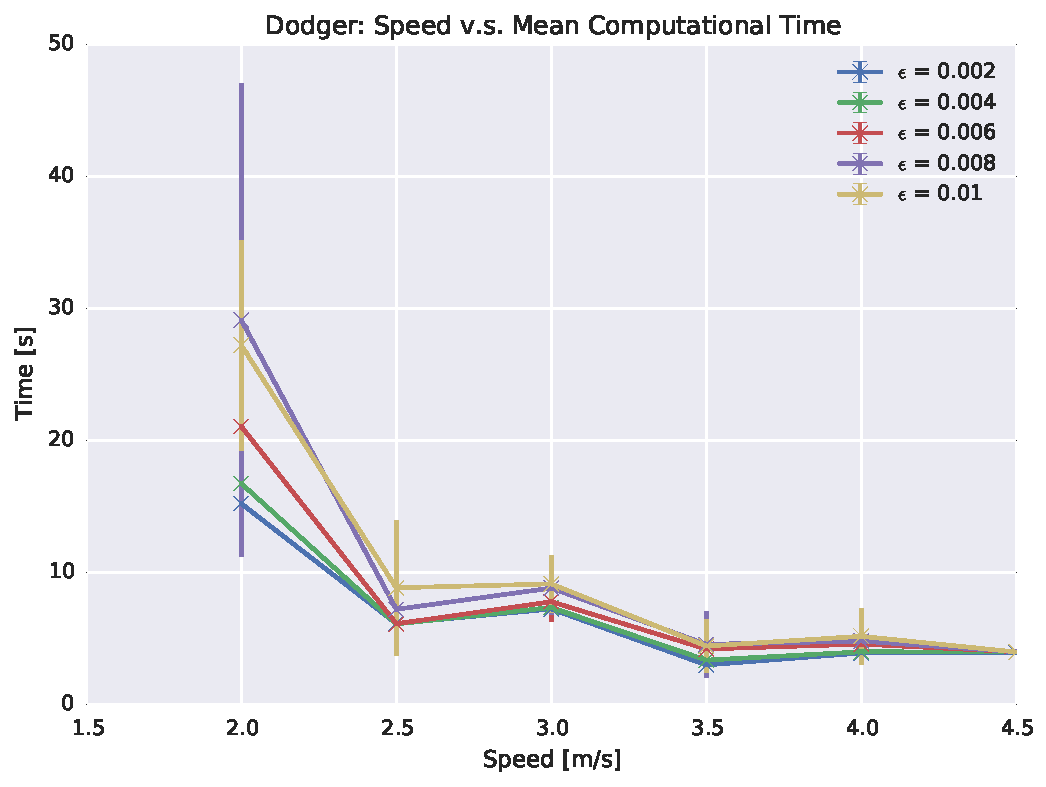
\includegraphics[width=0.48\linewidth]{figs/planner_small_mean_times_2}
    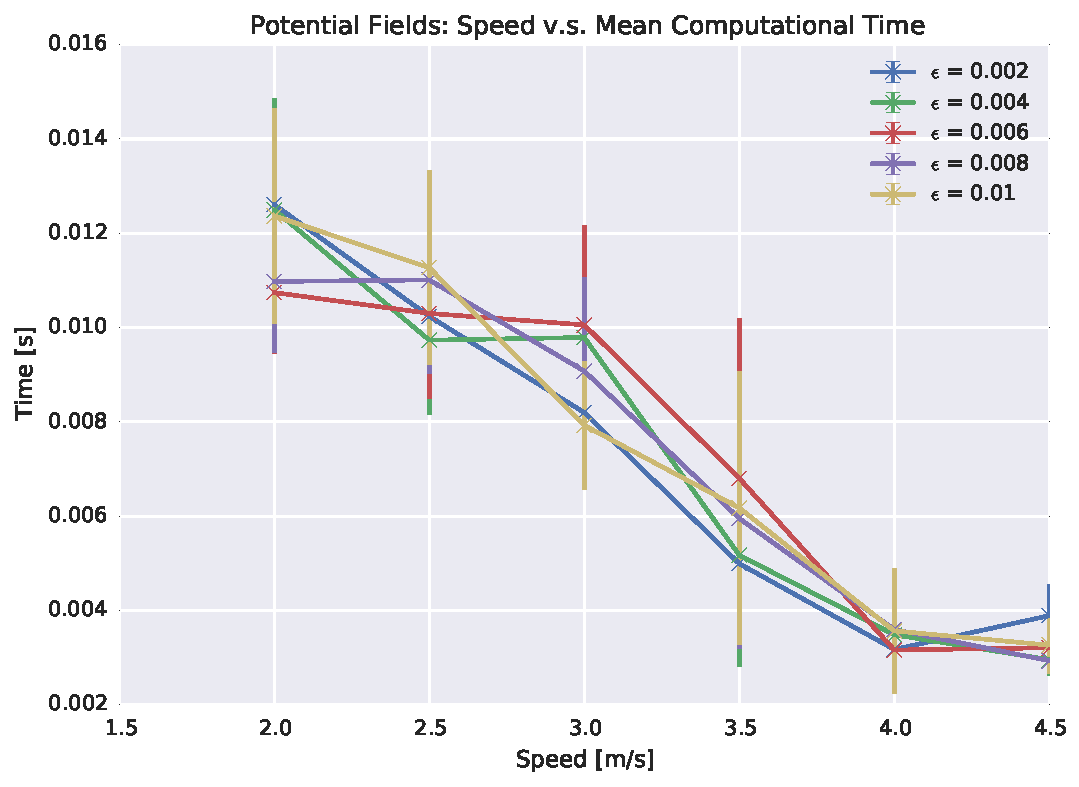
\includegraphics[width=0.48\linewidth]{figs/pf_small_mean_times_2}

    \caption{Plots showing how the computational to generate a path changes as
        the speed increases for various amounts of obstacle position
        uncertainties.  The horizontal axis represents the speed of the robot
        and the vertical axis represents the computational time to generate the
        path. The different lines on each plot represent experiments with
        differing amounts of noise and the error bars represent one standard
        deviation.  On the left is the graph for Dodger and on the right is the
    graph for the potential fields planner.}

\end{figure}

\begin{figure}[h!]
    \centering

    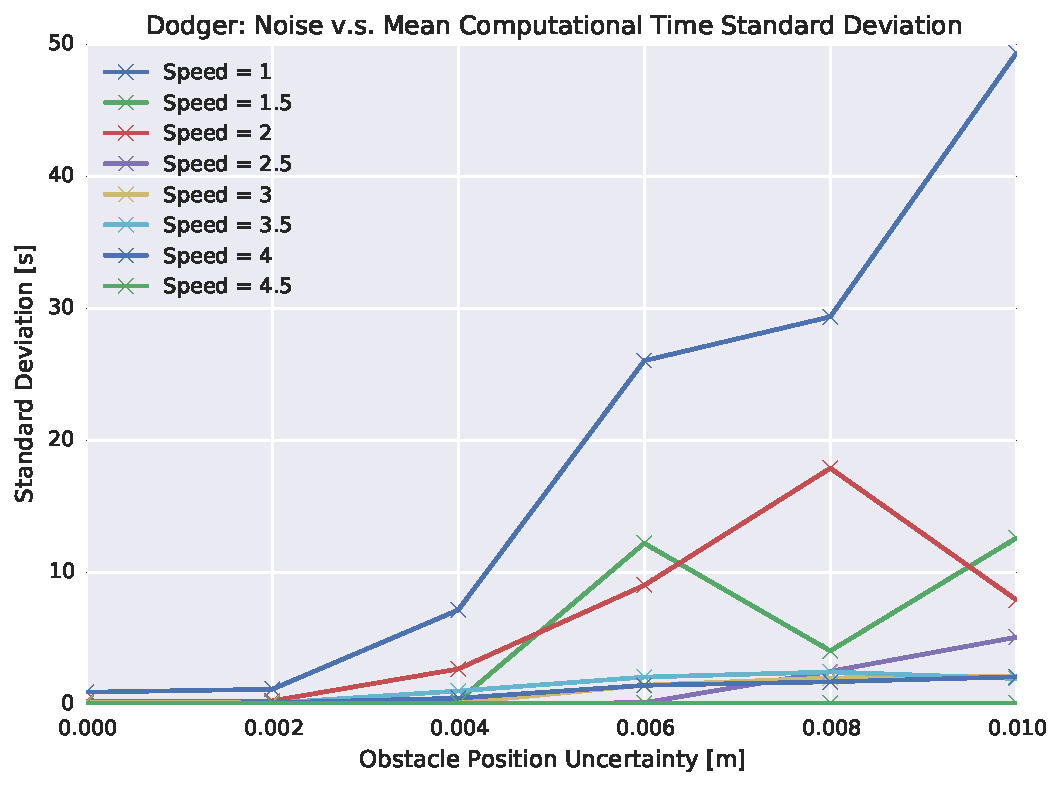
\includegraphics[width=0.48\linewidth]{figs/planner_std_avg_times_2}
    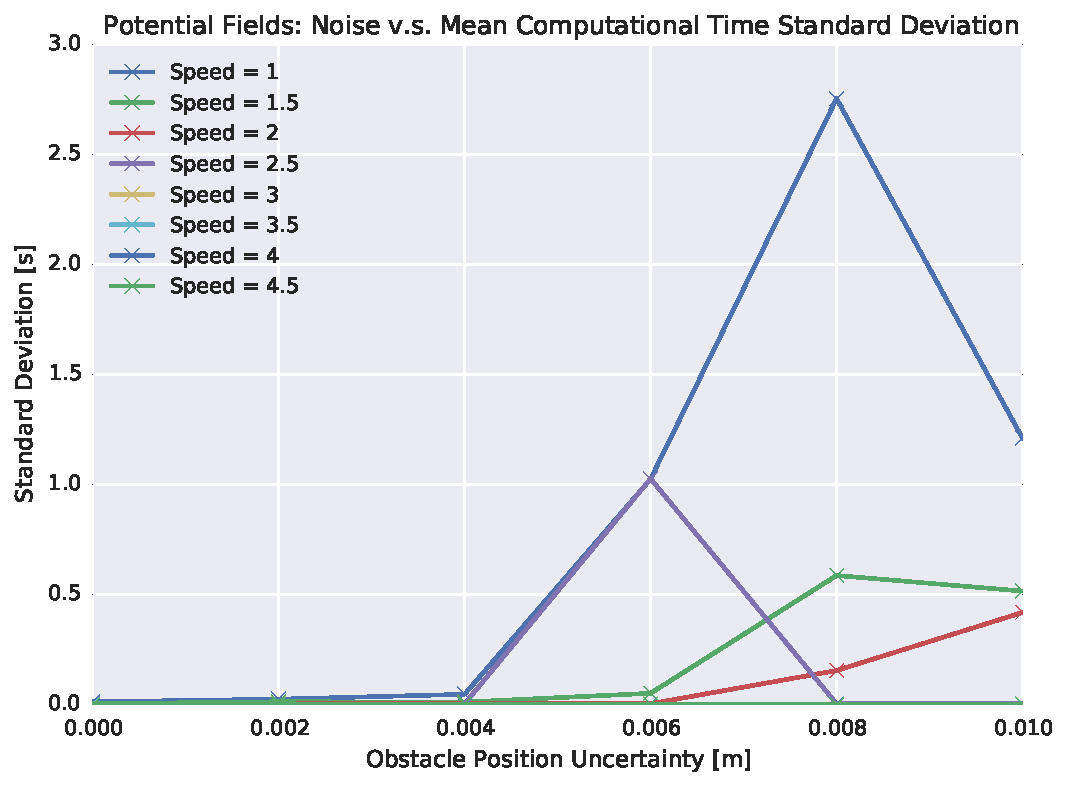
\includegraphics[width=0.48\linewidth]{figs/pf_std_avg_times_2}

    \caption{Plots showing how the standard deviation for the computational
        cost to generate a path changes as the noise injected into the obstacle
        trajectories increases.  The horizontal axis represents the amount of
        noise and the vertical axis represents the standard deviation. The
    different lines indicate different speeds that the robot was travelling. On
the left is the graph for Dodger and on the right is the graph for the
potential fields planner.}

\end{figure}


\end{document}
